\documentclass[10pt,a4paper]{article}
\usepackage[margin=2cm]{geometry}
\usepackage{graphicx}
\usepackage{booktabs}
\usepackage{amsmath,amssymb}
\usepackage{xcolor}
\usepackage{hyperref}
\usepackage{caption}
\usepackage{subcaption}
\usepackage{enumitem}
\usepackage{float}
\setlist{itemsep=1pt,parsep=0pt,topsep=2pt,partopsep=0pt,leftmargin=1.6em}
\setlength{\parindent}{0pt}
\setlength{\parskip}{4pt}
\hypersetup{colorlinks=true,linkcolor=blue!50!black,urlcolor=blue!50!black,citecolor=blue!50!black}
\graphicspath{{../figures/}}
\captionsetup{font=small,labelfont=bf}
\newcommand{\camz}{\texttt{cam00}}
\makeatletter\newcommand{\tabinput}[1]{\@@input #1 }\makeatother

\title{E9 247 Assignment 3: Temporal Interpolation with Dynamic 3D Gaussian Splatting\\[2pt]
\large TAD-GS vs.\ Spacetime Gaussians (STGS) vs.\ 4D Gaussian Splatting (4DGS)}
\author{Rohan, Soham, Sharan\\[2pt]
\small Code: \url{https://github.com/Sharkum/3DVision-Assignment3}}
\date{}

\begin{document}
\maketitle

%=====================================================================
\section{Setup}
%=====================================================================
\textbf{Data.} Neural 3D Video~\cite{dynerf}, \texttt{coffee\_martini}, frames 0--49, 18 cameras. All methods train on frames downsampled $4\times$ to $676\times507$. \textbf{Held-out camera:} \camz\ for every method and every $k$.

\textbf{Splits.} We train on frames $\{0,k,\ldots,48\}$ and test on the midpoints $\{k/2,3k/2,\ldots\}$, i.e.\ 25/13/7 training and 24/12/6 test frames for $k=2/4/8$. \emph{Setting A}: the 17 training cameras at the test frames (temporal interpolation only). \emph{Setting B}: \camz\ at the test frames (temporal + novel view).

\textbf{Methods.} All three are continuous in $t$, so test frames are rendered directly at their timestamps, and no interpolation rule is needed. \emph{(dev.)} marks a deviation from the method's defaults.
\begin{itemize}
\item \textbf{TAD-GS}~\cite{tadgs}: upstream \texttt{vikramsandu/TAD-GS} at \texttt{24c9f2a}.
\begin{itemize}
\item Hardware: NVIDIA RTX 3050 Ti Laptop (4\,GB), about 7.5 min per $k$
\item Iterations: 8\,000, batch 1 (dev.; default 30\,000)
\item Densification: every 200 iterations, from 400 to 4000, gradient threshold $3\times10^{-4}$ (dev.; default 500--17000, $2\times10^{-4}$)
\item Opacity reset: every 2000 iterations (dev.; default 3000)
\item Time model: VAD, TAT and TOW on; Fourier motion with $F=4$; TOW span and $\sigma_{\min}$ window 10 frames (dev.; default 50); span budget 70\%
\item Learning rates: position $2.6\times10^{-4}\to2.6\times10^{-6}$, features $2.5\times10^{-3}$, opacity 0.05, scaling $1.5\times10^{-3}$, rotation $10^{-3}$, temporal scale $3\times10^{-3}$
\item Final Gaussians: 182k / 189k / 223k for $k=2/4/8$
\end{itemize}
\item \textbf{STGS}~\cite{stgs}: upstream \texttt{oppo-us-research/SpacetimeGaussians} at \texttt{427abfc}, full model, authors' N3V configuration.
\begin{itemize}
\item Hardware: NVIDIA RTX A5000 (24\,GB), about 15 min per $k$
\item Iterations: 30\,000, batch 2 views
\item Densification: every 100 iterations, from 500 to 9000, gradient threshold $2\times10^{-4}$; opacity reset every 3000; error-guided sampling from 1600; at most 330k Gaussians
\item Time model: cubic polynomial motion, linear rotation, 9-D features with an MLP decoder
\item Learning rates: position $1.6\times10^{-4}\to1.6\times10^{-6}$, scaling $3\times10^{-3}$, opacity 0.05, rotation $10^{-3}$, features $2.5\times10^{-3}$, temporal centre $10^{-4}$, temporal scale 0.03
\item Image downsampling $4\times$ instead of $2\times$ (dev.)
\end{itemize}
\item \textbf{4DGS}~\cite{4dgs}: Wu et al., HexPlane + MLP deformation, authors' DyNeRF configuration.
\begin{itemize}
\item Hardware: NVIDIA GB10 (CUDA 13.0); 35 / 28 / 25 min for $k=2/4/8$
\item Iterations: 14\,000 (fine stage)
\item Timestamps normalised as $f/49$ (dev.: the loader divided by the full 300-frame length)
\item Final Gaussians: 85k / 91k / 83k for $k=2/4/8$
\end{itemize}
\end{itemize}

\textbf{Metrics.} PSNR, SSIM and LPIPS-Alex at $676\times507$, averaged over the test images, for all methods.

%=====================================================================
\section{Dynamic-region mask}\label{sec:mask}
%=====================================================================
The mask is computed from the ground-truth video, one per camera:
\begin{enumerate}
\item Compute dense optical flow (Farneb\"ack) over the 50 frames, keeping only forward--backward-consistent flow.
\item Average the flow magnitude over time, giving one motion map per camera.
\item Threshold the map with Otsu's method (0.38\,px on \camz).
\item Take the smallest bounding box around the pixels above the threshold (9.2\% of the image on \camz).
\end{enumerate}
The same box is used for all frames, all $k$ and all three methods. Dynamic-region metrics are computed inside the box (Fig.~\ref{fig:mask}).

\begin{figure}[H]
\centering
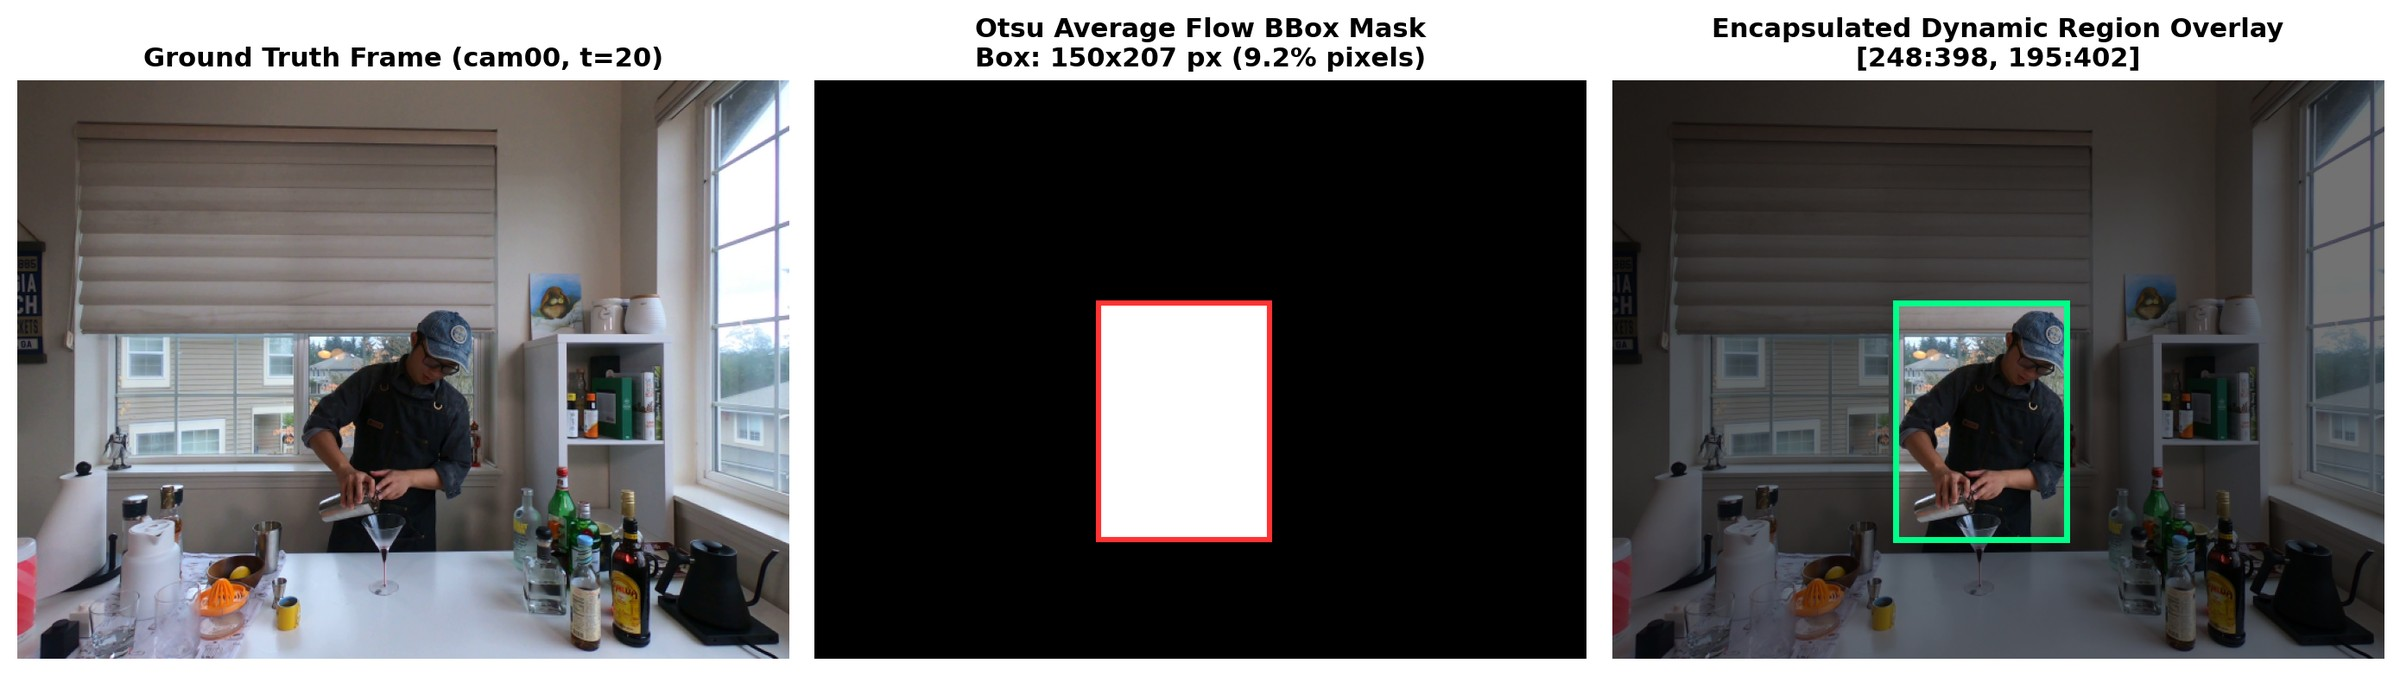
\includegraphics[width=0.75\linewidth]{tadgs_mask_cam00.jpg}
\caption{Dynamic-region mask on \camz\ ($t=20$): ground truth, mask, overlay.}
\label{fig:mask}
\end{figure}

%=====================================================================
\section{Results}
%=====================================================================
\subsection{Quality on test frames}
\begin{table}[H]
\centering\small
\caption{Full-image quality on test frames. Bold: best.}
\label{tab:full}
\begin{tabular}{cc ccc ccc ccc}
\toprule
& & \multicolumn{3}{c}{TAD-GS} & \multicolumn{3}{c}{STGS} & \multicolumn{3}{c}{4DGS} \\
\cmidrule(lr){3-5}\cmidrule(lr){6-8}\cmidrule(lr){9-11}
Set. & $k$ & PSNR$\uparrow$ & SSIM$\uparrow$ & LPIPS$\downarrow$ & PSNR$\uparrow$ & SSIM$\uparrow$ & LPIPS$\downarrow$ & PSNR$\uparrow$ & SSIM$\uparrow$ & LPIPS$\downarrow$ \\
\midrule
\tabinput{../tables/table_full.tex}
\bottomrule
\end{tabular}
\end{table}

\begin{table}[H]
\centering\small
\caption{Dynamic-region quality on test frames. Bold: best.}
\label{tab:dyn}
\begin{tabular}{cc ccc ccc ccc}
\toprule
& & \multicolumn{3}{c}{TAD-GS} & \multicolumn{3}{c}{STGS} & \multicolumn{3}{c}{4DGS} \\
\cmidrule(lr){3-5}\cmidrule(lr){6-8}\cmidrule(lr){9-11}
Set. & $k$ & PSNR$\uparrow$ & SSIM$\uparrow$ & LPIPS$\downarrow$ & PSNR$\uparrow$ & SSIM$\uparrow$ & LPIPS$\downarrow$ & PSNR$\uparrow$ & SSIM$\uparrow$ & LPIPS$\downarrow$ \\
\midrule
\tabinput{../tables/table_dyn.tex}
\bottomrule
\end{tabular}
\end{table}

\subsection{Per-frame PSNR, $k=8$}
\begin{figure}[H]
\centering
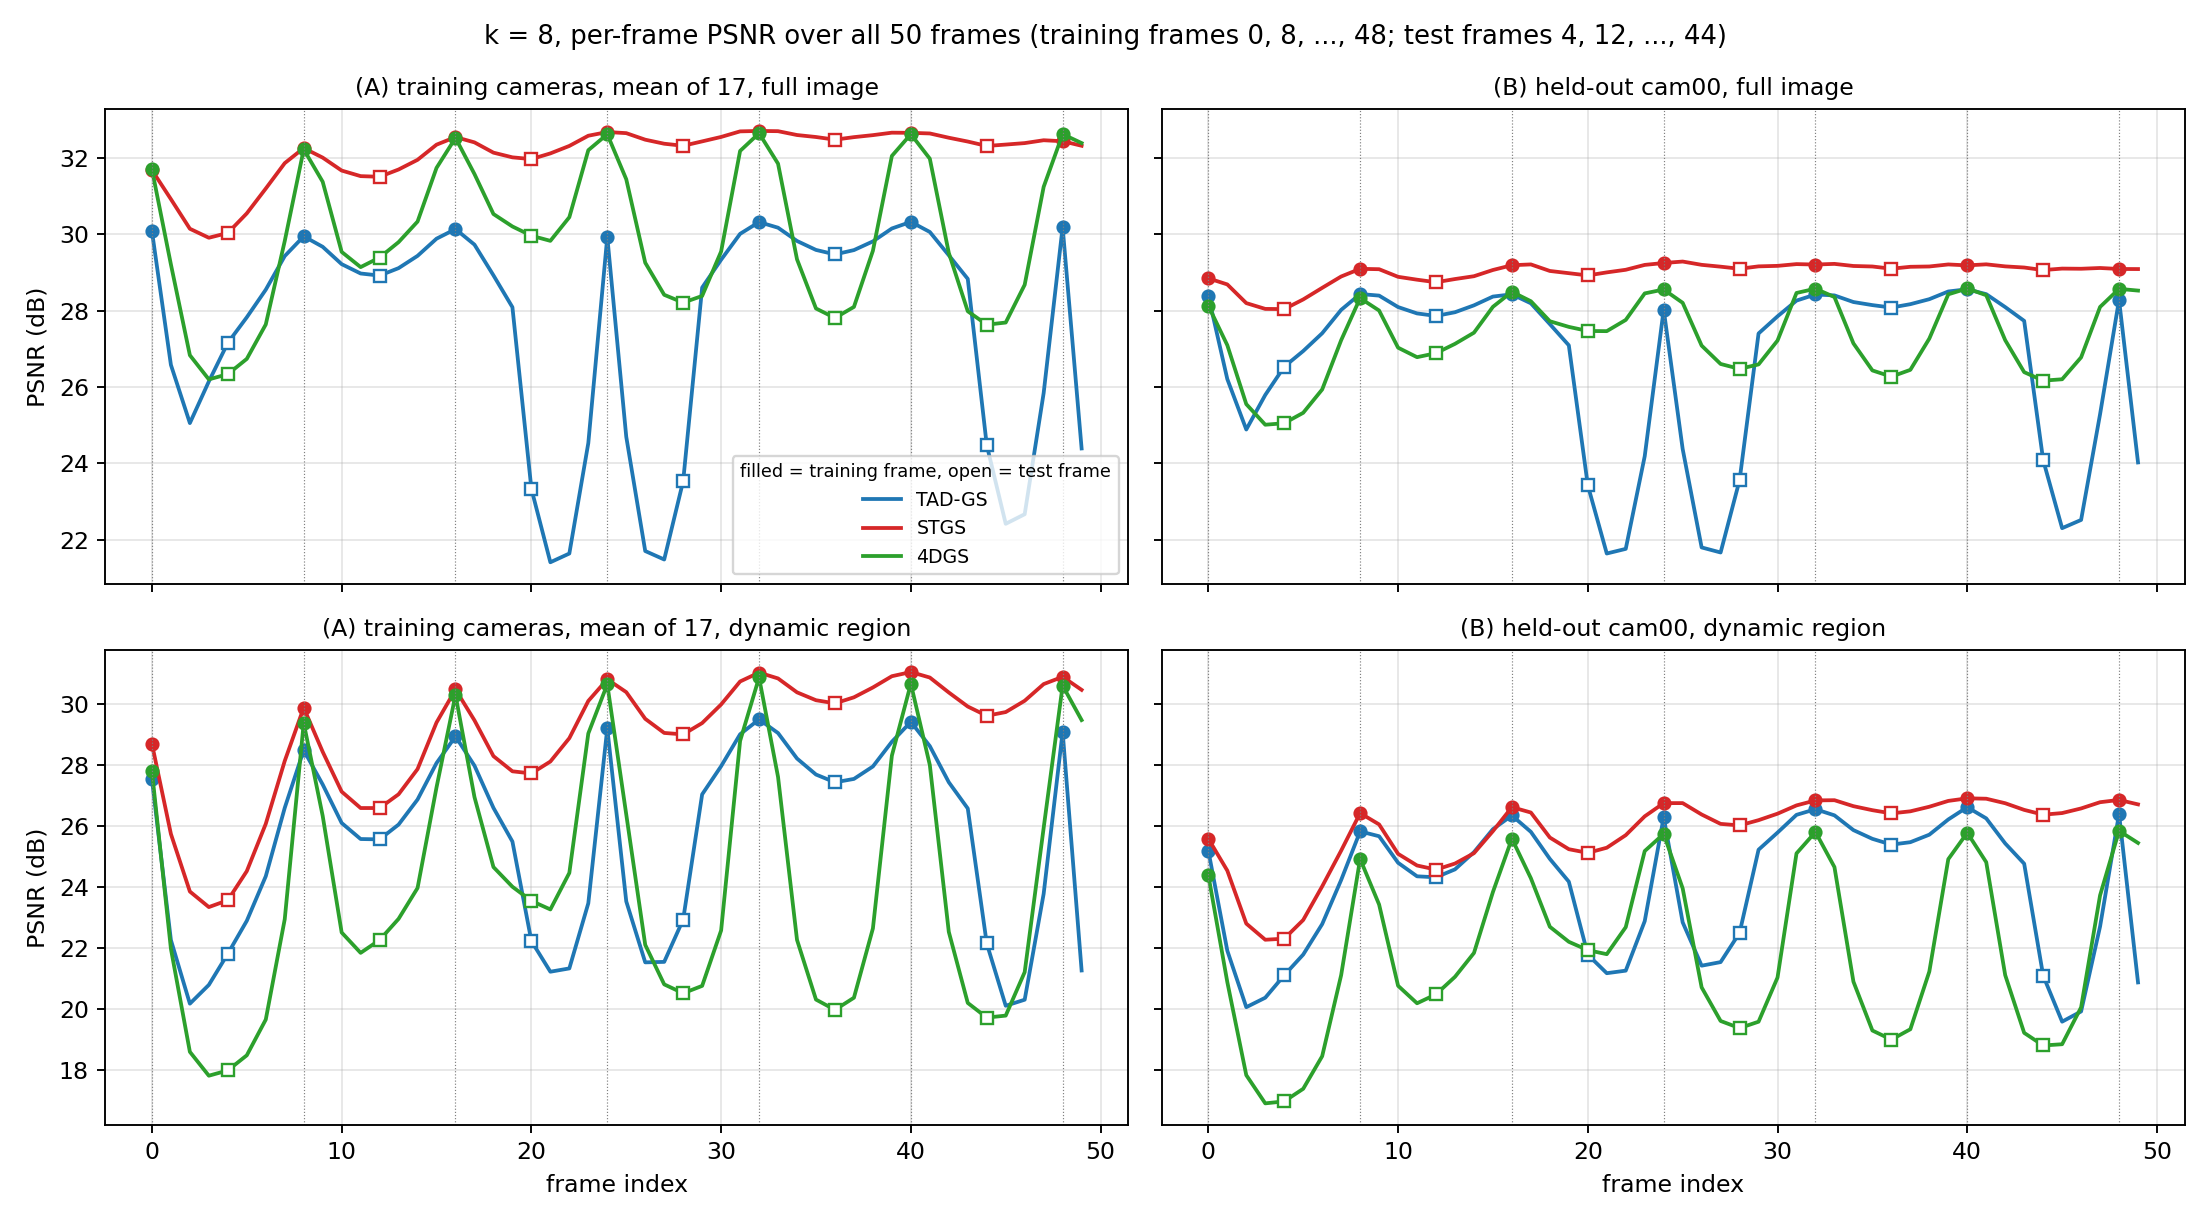
\includegraphics[width=\linewidth]{fig_perframe_k8_uniform.png}
\caption{Per-frame PSNR at $k=8$ over all 50 frames. Filled: training frames; open: test frames.}
\label{fig:pfu}
\end{figure}

\begin{figure}[H]
\centering
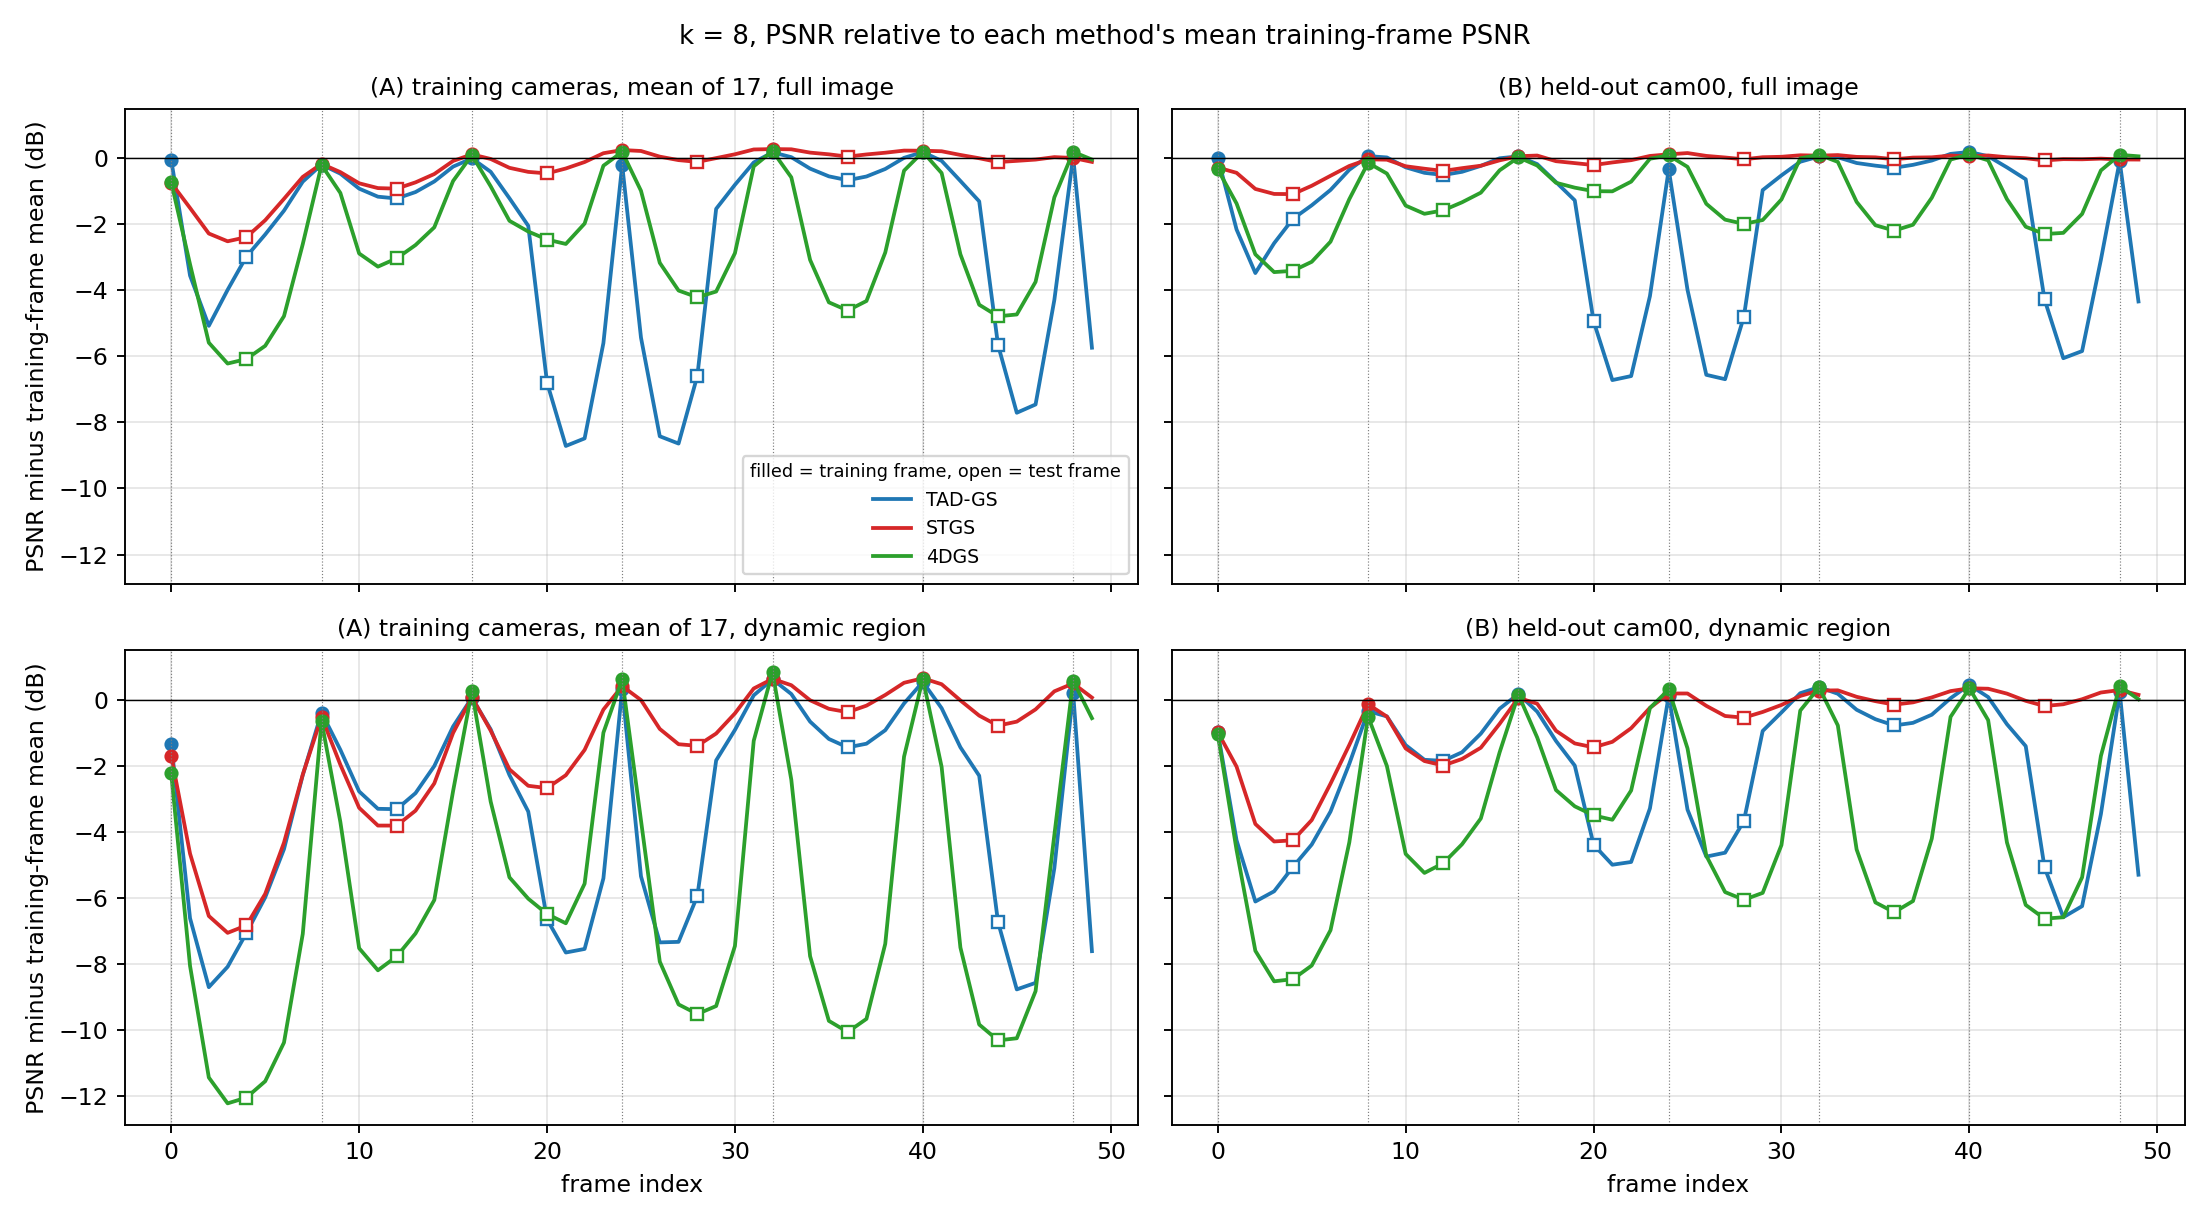
\includegraphics[width=\linewidth]{fig_perframe_k8_relative.png}
\caption{Fig.~\ref{fig:pfu} relative to each method's mean training-frame PSNR. STGS shows a shallow sawtooth, deepest in the fast frames 0--16. 4DGS shows a deep, regular sawtooth across the whole sequence. TAD-GS follows STGS in frames 8--19 and 29--43, and collapses by 4--9\,dB around frames 0, 24 and 48.}
\label{fig:pfrel}
\end{figure}

\begin{table}[H]
\centering\small
\caption{$k=8$: mean PSNR at training vs.\ test frames; ``cost'' is the difference.}
\label{tab:trtest}
\begin{tabular}{l cc c cc c}
\toprule
& \multicolumn{3}{c}{A: training cameras} & \multicolumn{3}{c}{B: \camz} \\
\cmidrule(lr){2-4}\cmidrule(lr){5-7}
& train & test & cost & train & test & cost \\
\midrule
\tabinput{../tables/table_trtest.tex}
\bottomrule
\end{tabular}
\end{table}

\begin{figure}[H]
\centering
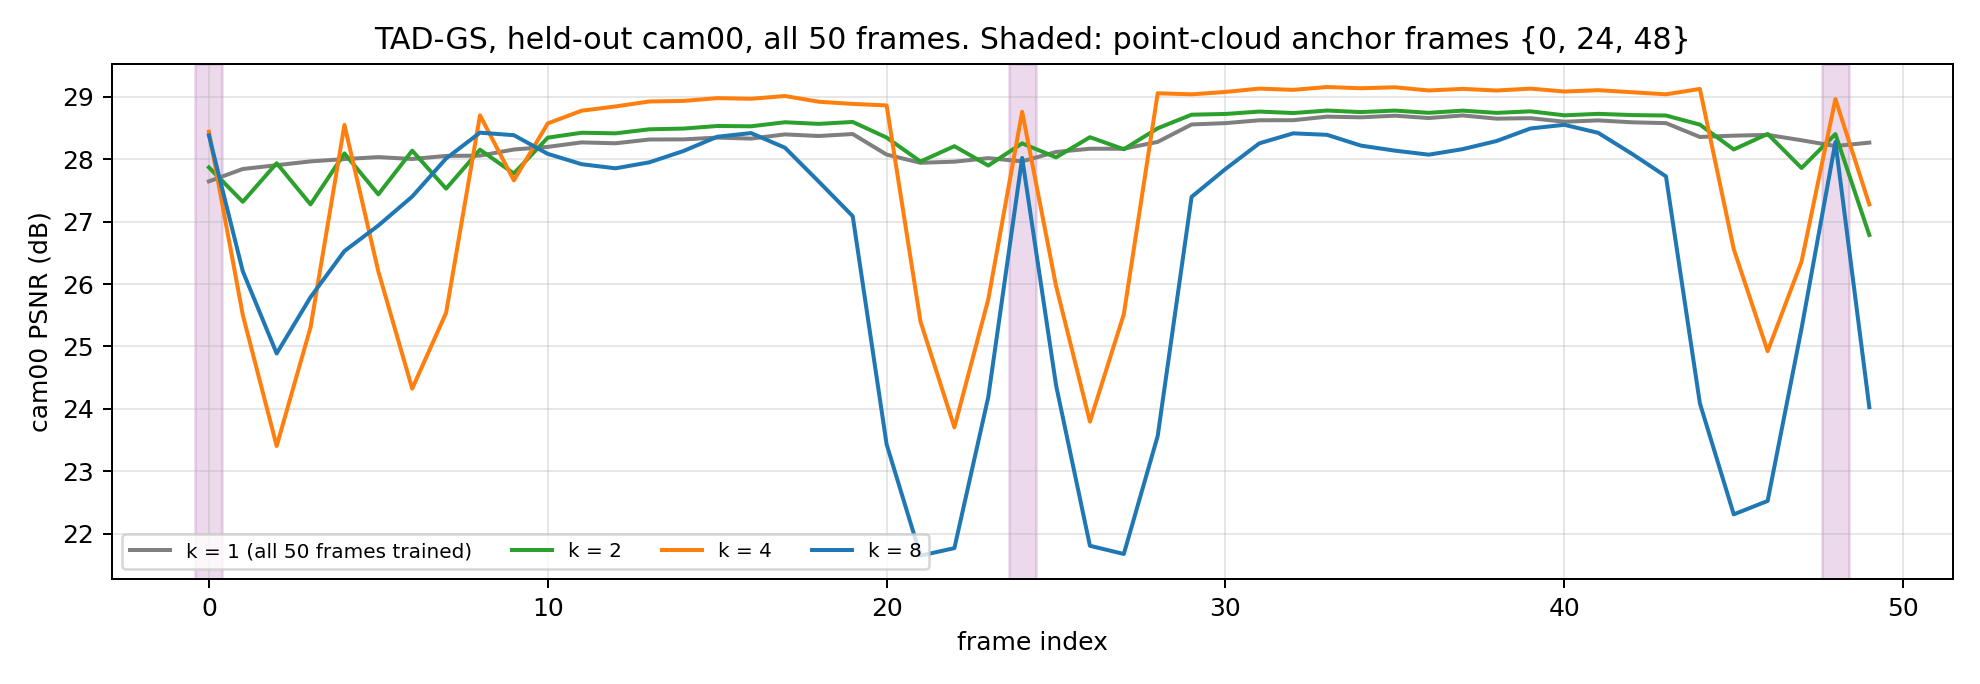
\includegraphics[width=\linewidth]{fig_tadgs_perframe_cam00_allk.png}
\caption{TAD-GS on \camz, all frames, $k\in\{1,2,4,8\}$. The drops sit within $\pm5$ frames of the anchor frames $\{0,24,48\}$ for both $k=4$ and $k=8$.}
\label{fig:tadallk}
\end{figure}

\subsection{Visual results}
All methods are shown on \camz\ at $676\times507$, on the test frame with the most ground-truth motion for each $k$ ($t=1/2/4$ for $k=2/4/8$). The crop is the same $160\times160$ region at the flow peak for every method, and the error map is the mean absolute RGB error on a fixed 0--0.25 scale.

\begin{figure}[H]
\centering
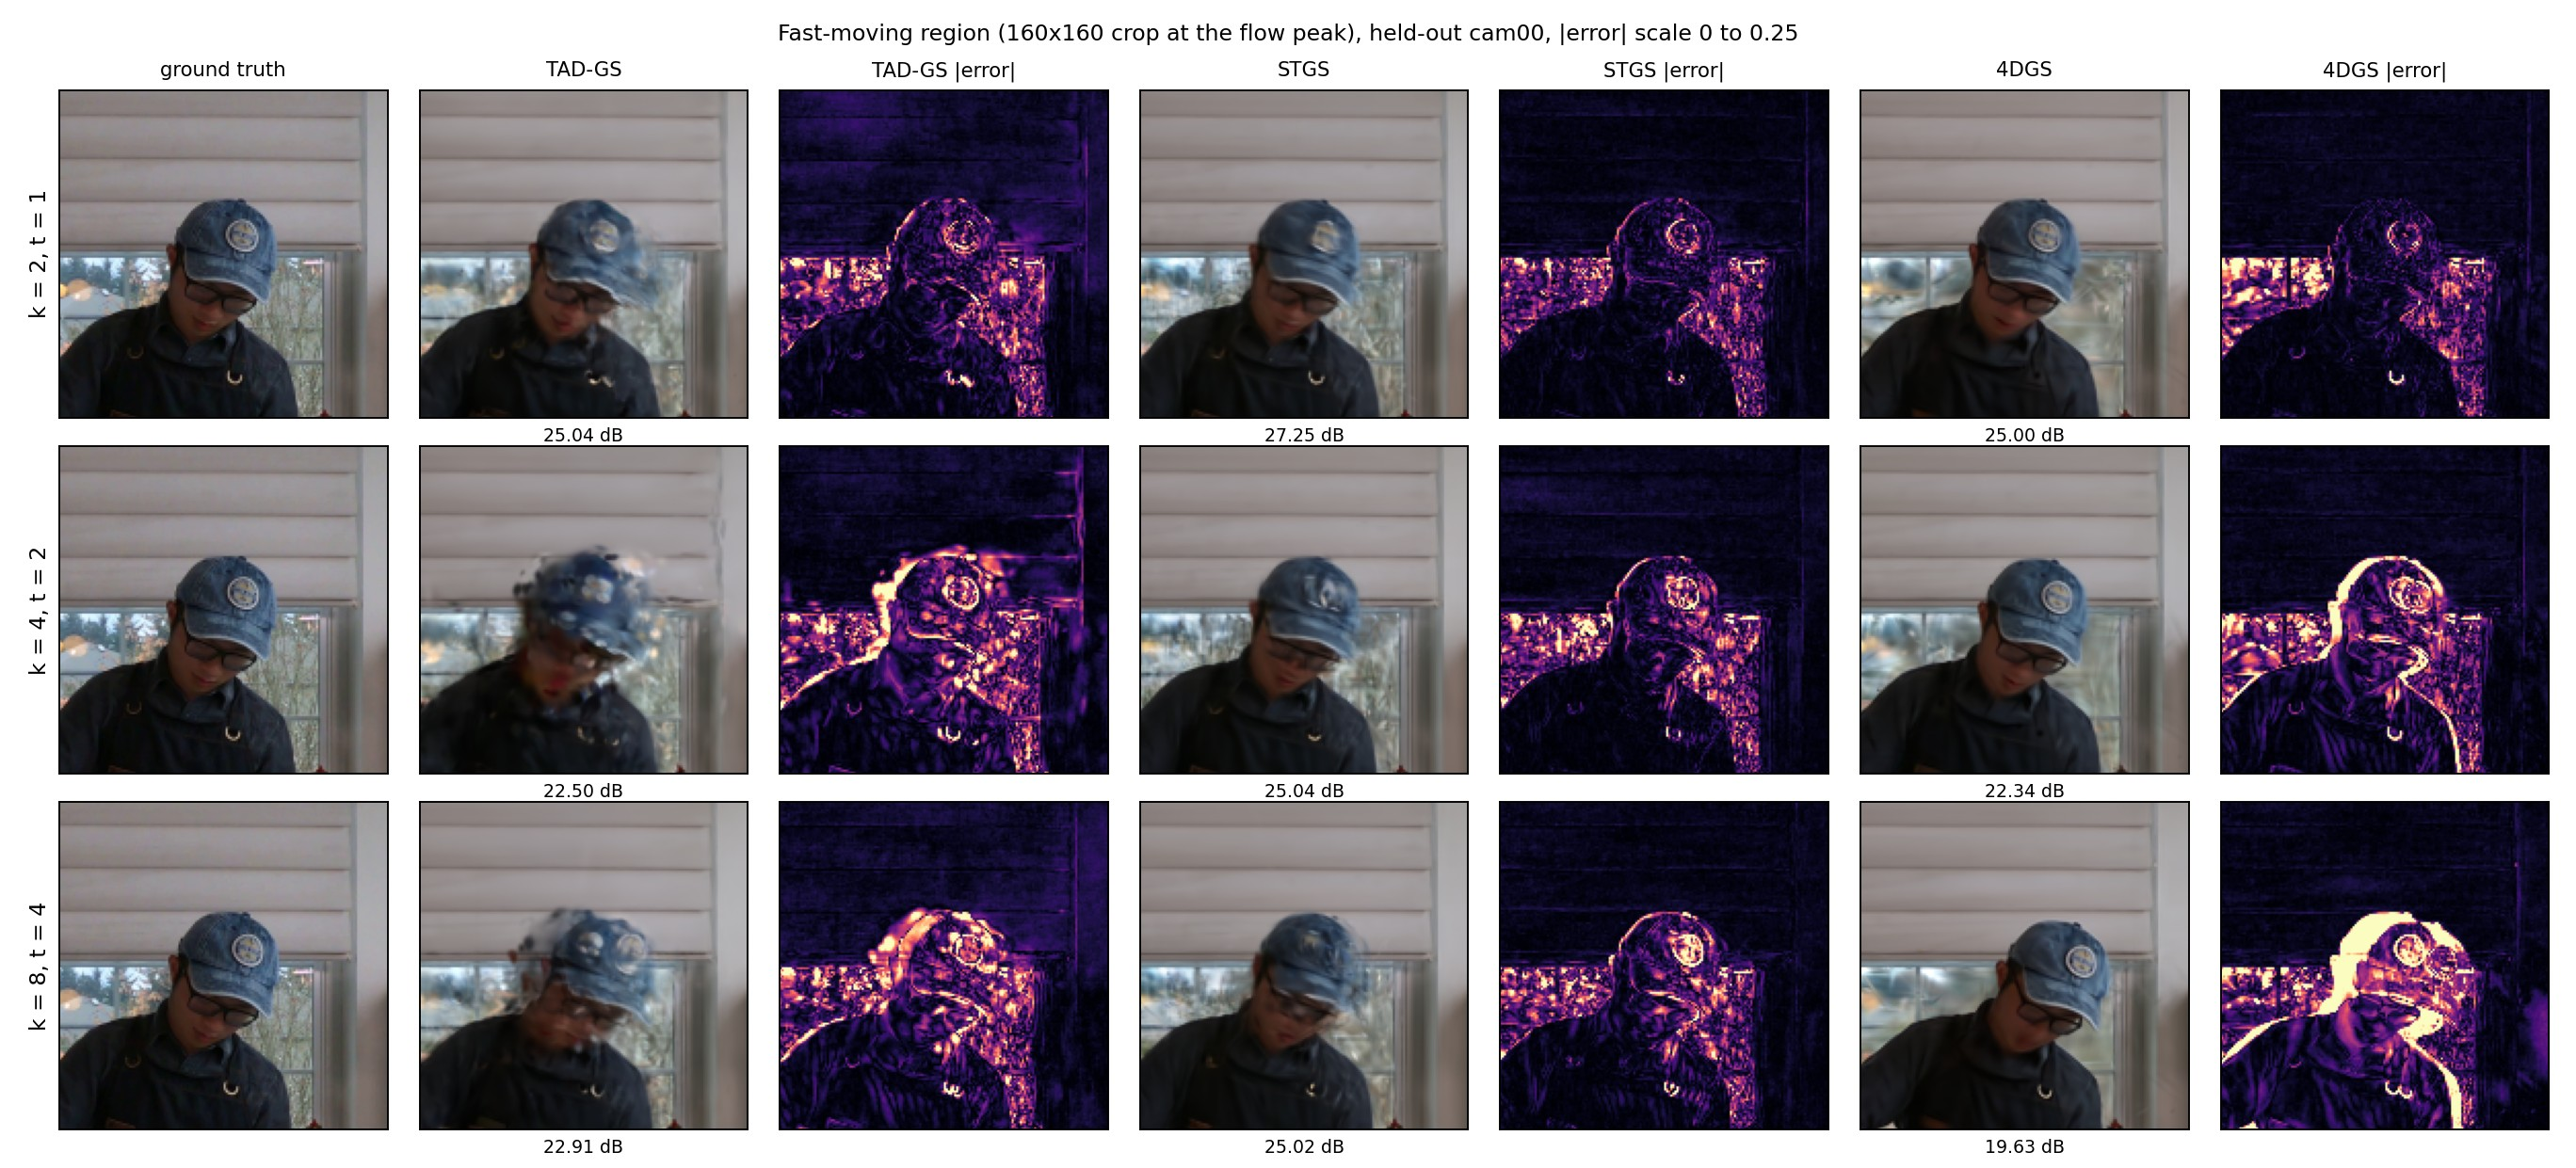
\includegraphics[width=\linewidth]{visual_uniform_crops.jpg}
\caption{Fast-moving region, all methods and $k$, with crop PSNR. STGS blurs and then doubles the cap and face. TAD-GS breaks them into floaters at $k=4,8$. 4DGS keeps them sharp but displaced.}
\label{fig:viscrop}
\end{figure}

\begin{figure}[H]
\centering
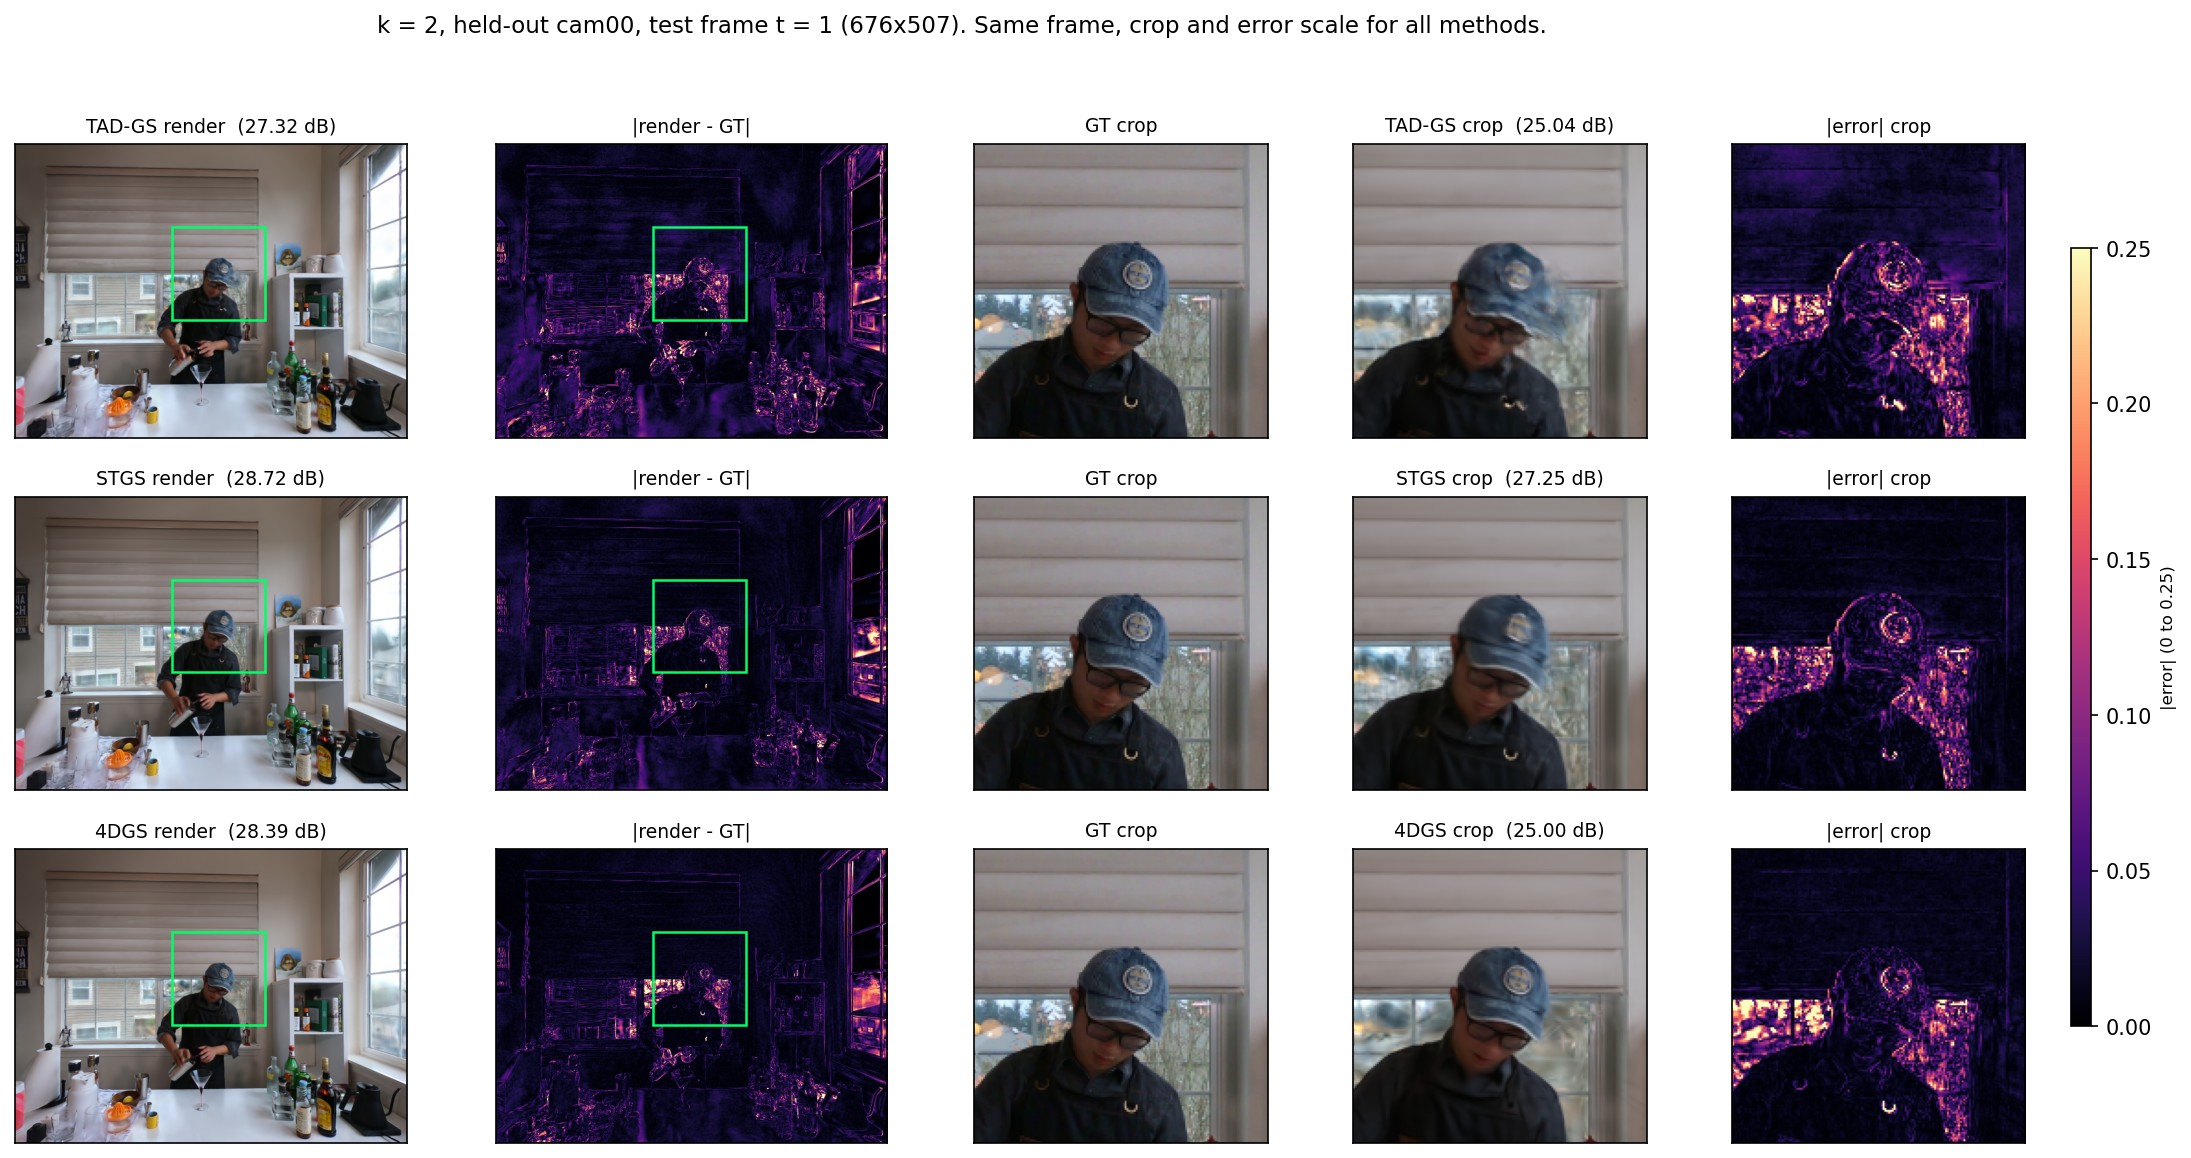
\includegraphics[width=\linewidth]{visual_uniform_k2.jpg}
\caption{$k=2$, $t=1$: full frame, error map and crop.}
\label{fig:vis2}
\end{figure}
\begin{figure}[H]
\centering
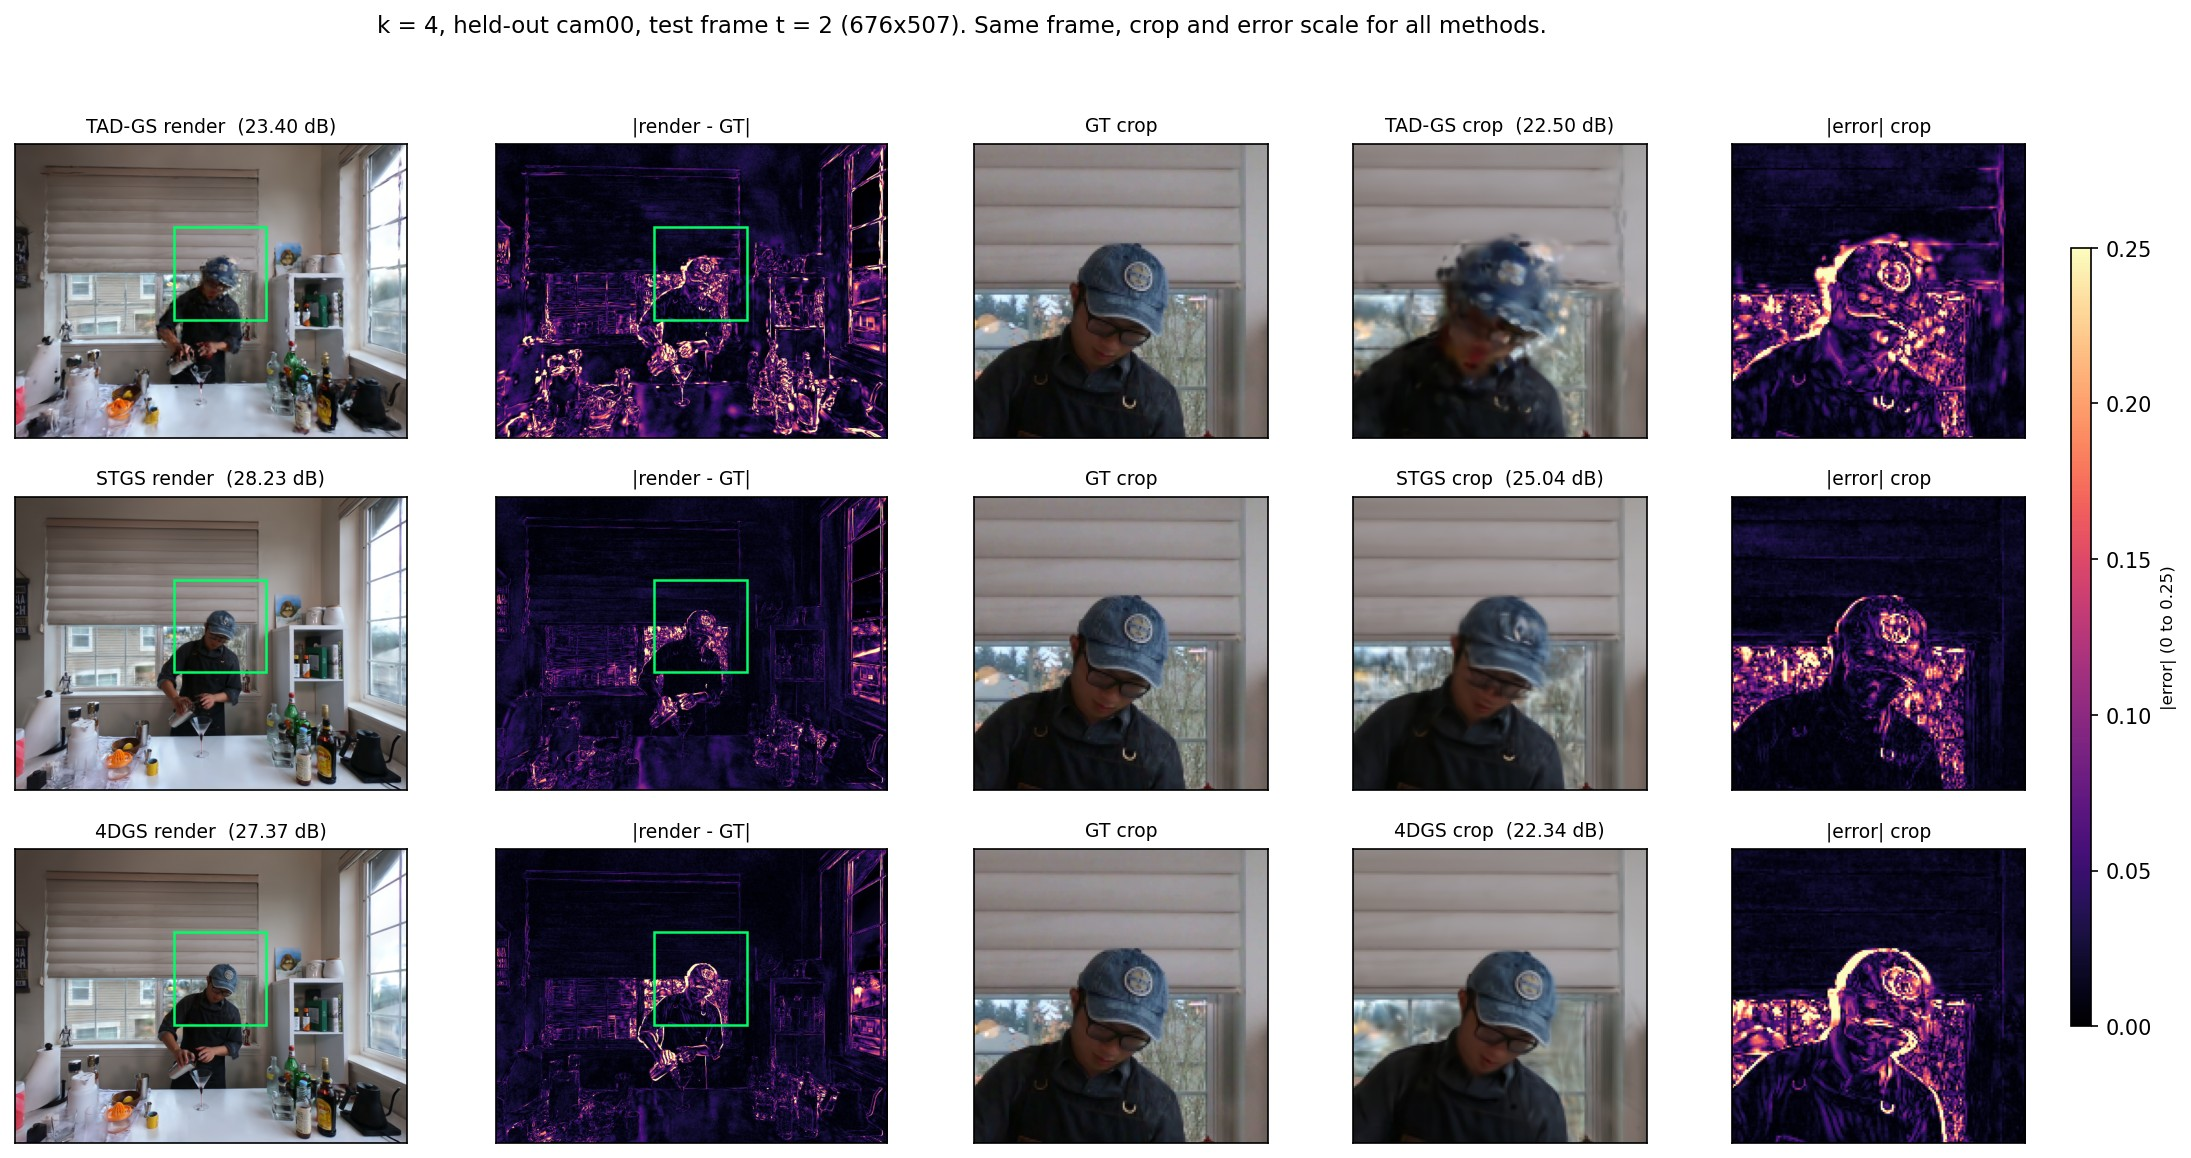
\includegraphics[width=\linewidth]{visual_uniform_k4.jpg}
\caption{$k=4$, $t=2$. The TAD-GS error spreads to static edges, since $t=2$ is inside its anchor-0 window.}
\label{fig:vis4}
\end{figure}
\begin{figure}[H]
\centering
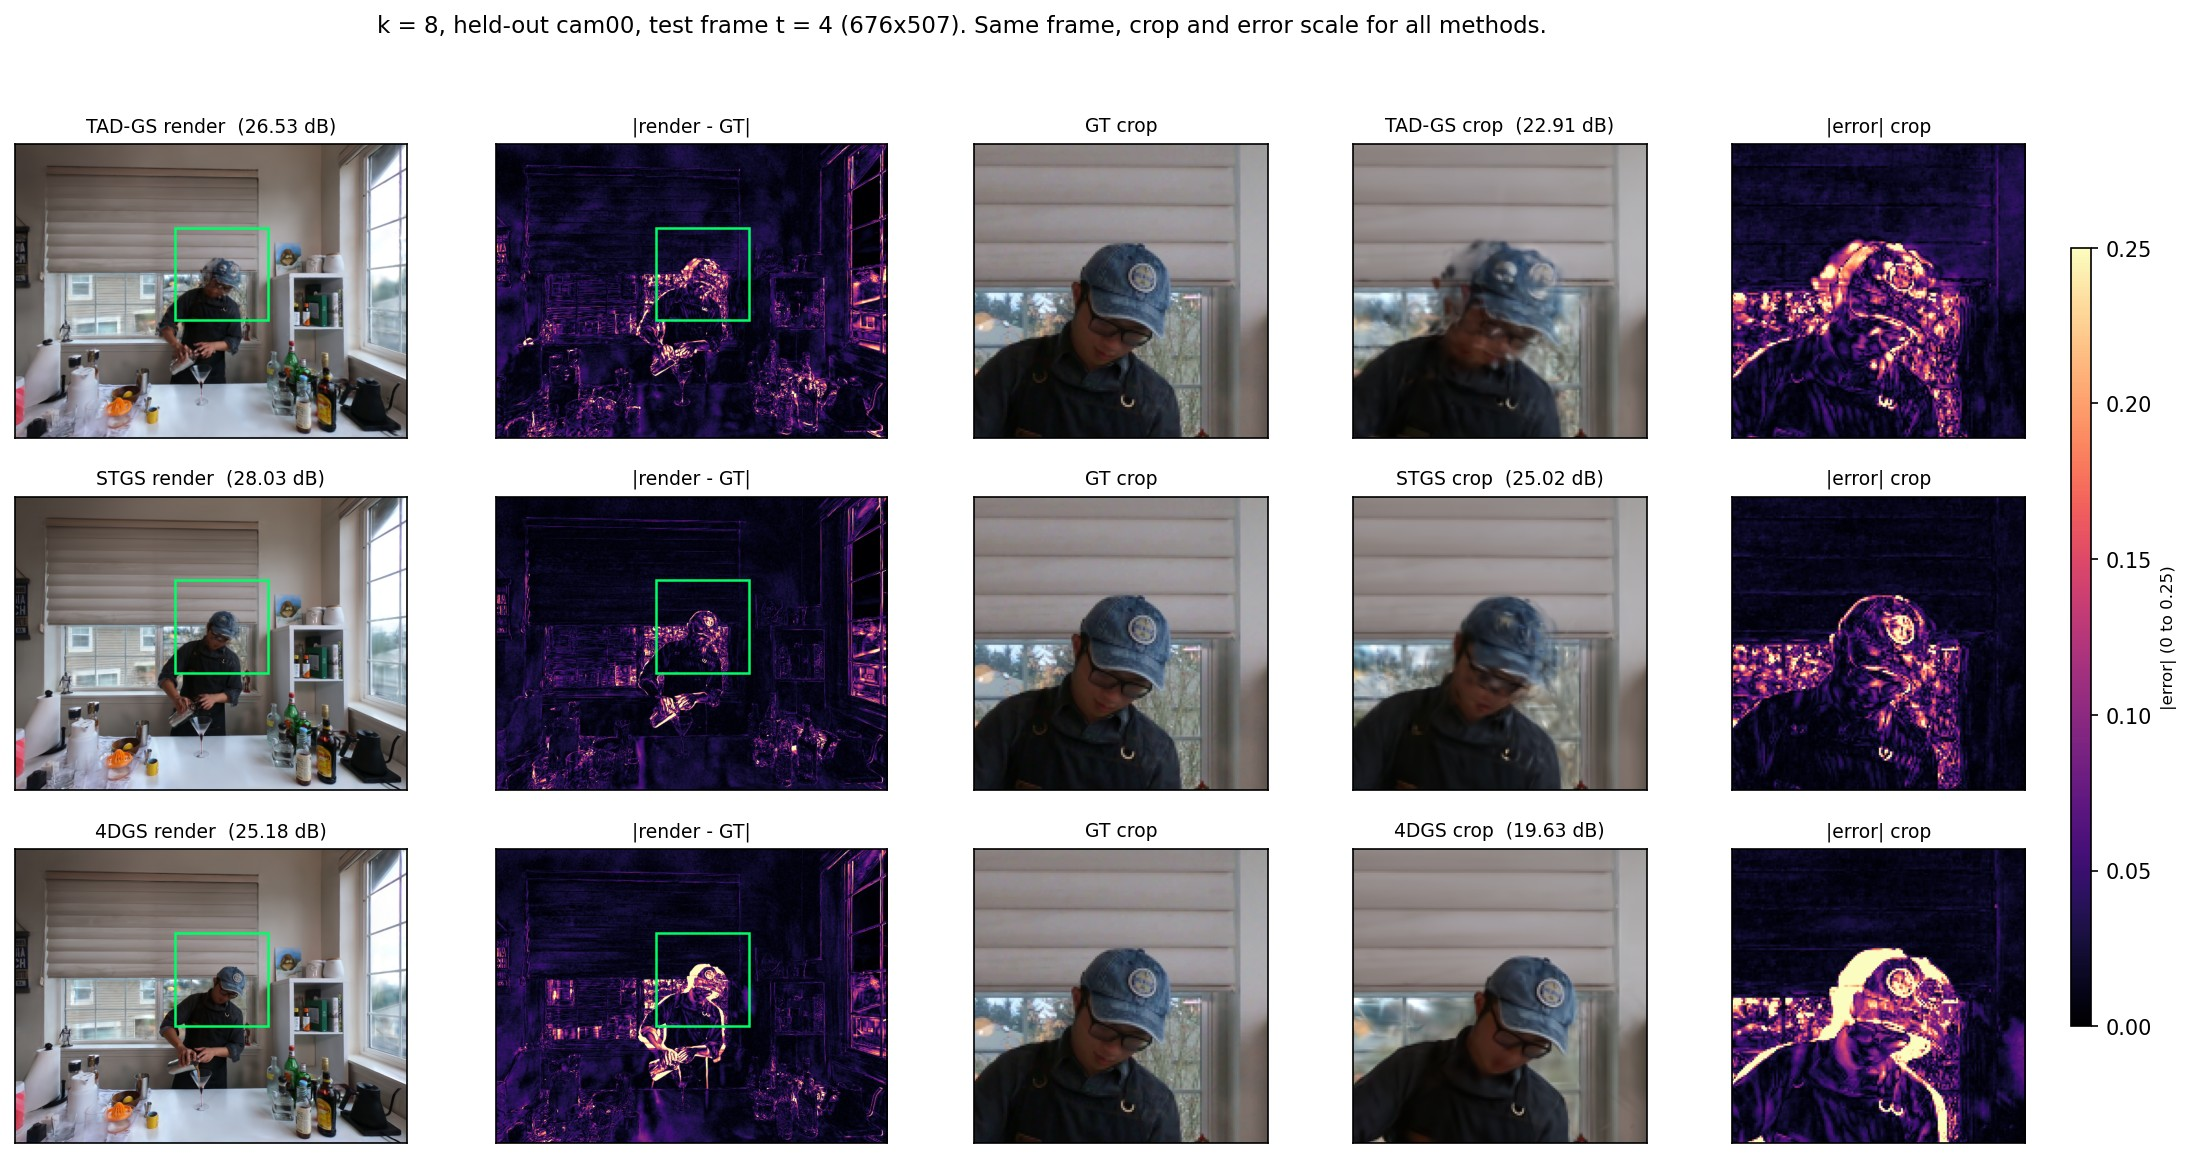
\includegraphics[width=\linewidth]{visual_uniform_k8.jpg}
\caption{$k=8$, $t=4$. The 4DGS error forms a thick outline around the arm, shaker and head, i.e.\ misplacement rather than blur.}
\label{fig:vis8}
\end{figure}

%=====================================================================
\section{Answers}
%=====================================================================
\subsection*{Q1. How does each method represent time, and what does that predict?}
The three methods fall into two families. STGS and TAD-GS give every Gaussian its own lifetime and its own path through the scene. 4DGS keeps one set of Gaussians for the whole video and moves them all with a single learned deformation.
\begin{itemize}
\item \textbf{STGS} treats each Gaussian as a short-lived object. It is most visible at one moment, fades in before it and out after it, and follows its own smooth path while it is visible. Fast motion is covered by many short-lived Gaussians that take over from each other.
\emph{Prediction:} slow motion should interpolate well, because a smooth path that fits the training frames also fits the frames in between. Over a large gap, fast motion should blur or appear twice. The paths are fitted only at training frames, and short-lived Gaussians fade out between them, so the render blends the neighbouring poses instead of tracking the motion.
\item \textbf{TAD-GS} uses the same representation as STGS, with three changes:
\begin{itemize}
\item Each Gaussian's clock runs faster in a window around the moment it is most visible (TOW; $\pm5$ frames in our runs), so it can change quickly there.
\item It can fade in and out at different rates.
\item Its path is a sum of a few waves (a Fourier series) instead of a polynomial curve.
\end{itemize}
All Gaussians are centred on the anchor frames $\{0,24,48\}$, and those added during training keep their parent's centre. The paper's main contribution (VAD and TAT) decides where new Gaussians are added; it does not change how time is represented.
\emph{Prediction:} the paths are bounded, so nothing should blow up at an unseen time. Near the anchor frames, however, motion and opacity change quickly from frame to frame, and sparse training frames may not be enough to pin them down there.
\item \textbf{4DGS} does not store time in the Gaussians. A learned deformation field, a feature grid over space and time read by a small network, tells each Gaussian where to move at time $t$.
\emph{Prediction:} objects can move but cannot appear or disappear. The grid's time axis is supervised only at training times, so between them the motion should change smoothly and symmetrically, blending the neighbouring poses.
\end{itemize}

\subsection*{Q2. How does quality change with $k$, and when does each method fail?}
All three get worse as $k$ grows, but at different rates and in different ways.
\begin{itemize}
\item \textbf{STGS} loses the least. In Setting A its full-image PSNR goes from 33.29 to 32.86 to 31.76\,dB, and the dynamic region from 31.19 to 30.30 to 27.75\,dB. Most of the drop at $k=8$ comes from the first few frames, where the bartender moves fastest. At $t=4$ the dynamic-region PSNR is 23.6\,dB, compared with 28.7 and 29.9\,dB at the neighbouring training frames 0 and 8, and the cap and face appear twice. This is what we expected from its short-lived Gaussians.
\item \textbf{4DGS} starts close to STGS at $k=2$ (32.43 vs.\ 33.29\,dB in A) but falls off quickly, to 31.13 and then 28.22\,dB, and from 29.64 to 20.66\,dB in the dynamic region. At $k=8$ it reconstructs the training frames as well as STGS does (32.41\,dB), yet its test frames are 4.2\,dB below its own training frames (3.5\,dB below STGS on the same test frames), and 9.4\,dB below in the dynamic region. This is the largest train--test loss of the three methods in Setting A (TAD-GS: 4.0\,dB) and in the dynamic region in both settings. The per-frame curve dips smoothly and symmetrically between training frames, as we predicted, but the renders do not look like a blend of two poses: the hands and the head are sharp but in the wrong place (Fig.~\ref{fig:vis8}). Our reading is that the HexPlane time features fit the training timestamps closely, and at an unseen time the deformation stays close to one of the nearby training poses instead of moving between them.
\item \textbf{TAD-GS} is the lowest of the three at every $k$, falling from 30.14 to 27.85 to 26.15\,dB in A. Its 4.0\,dB drop is close to that of 4DGS (4.2\,dB), but it is not spread evenly over the sequence. Away from the anchor frames it holds up much better: the $k=4$ test frames between 10 and 42 score 30.1--30.9\,dB, against 23.3--25.1\,dB for the test frames near the anchors, though still about 2.4\,dB below STGS (32.6--33.3\,dB) on the same frames. At $k=8$, over all 50 frames, \camz\ PSNR averages 23.0\,dB within three frames of anchors 24 and 48, against 27.5\,dB elsewhere, and floaters appear across the whole image, background included. We think this comes from our choice of a 10-frame TOW span, down from the default 50 (not yet tested). Every Gaussian's temporal centre is one of the anchor frames, so the warped region of the time axis sits exactly on those frames. There the Fourier motion changes too quickly to be pinned down by training frames that are 4--8 frames apart. This explains where the dips are and how wide they are, why they are small at $k=2$, and why there are none at $k=1$.
\end{itemize}

\subsection*{Q3. Is there a dynamic vs.\ static gap, and does it depend on the method?}
Yes, and where the error goes depends on the method. The error maps (Figs.~\ref{fig:vis2}--\ref{fig:vis8}) show it directly:
\begin{itemize}
\item \textbf{4DGS:} the error is concentrated on the bartender, as a bright outline around the arm, shaker and head, while the static background stays dark (Fig.~\ref{fig:vis8}). Tables~\ref{tab:full} and~\ref{tab:dyn} agree: from $k=2$ to 8 in A, the dynamic-region PSNR falls by 9.0\,dB but the full image only by 4.2\,dB.
\item \textbf{STGS:} the error is also mostly on the moving cap and face, and it is lower everywhere than for the other two methods. Some of the gap is present even at training frames (about 2\,dB in A at $k=8$), so not all of it is temporal.
\item \textbf{TAD-GS:} the error spreads to static edges, such as the bottles and window frames, whenever the test frame falls inside an anchor window (Fig.~\ref{fig:vis4}). Its full-image and dynamic-region PSNR fall by about the same amount from $k=2$ to 8 (4.0 and 4.1\,dB in A), because its failure hits static and moving pixels alike.
\end{itemize}
For STGS and 4DGS, full-image metrics hide most of the temporal error.

\subsection*{Q4. Does the held-out camera behave differently?}
Yes. Setting B is below A for every method and every $k$, but the A$-$B gap shrinks as $k$ grows, because \camz\ loses less PSNR with $k$ than the training cameras do:
\begin{itemize}
\item \textbf{STGS:} \camz\ is 4.4\,dB below A at $k=2$ and 2.9\,dB below at $k=8$. Full-image PSNR on \camz\ is nearly flat in $k$ (28.91/28.90/28.82\,dB), while A drops by 1.5\,dB. The temporal effect shows only in the dynamic region (27.29$\to$25.13\,dB).
\item \textbf{4DGS:} \camz\ is 4.0\,dB below A at $k=2$. It drops by 2.0\,dB with $k$, against 4.2\,dB for A, so the gap shrinks to 1.8\,dB.
\item \textbf{TAD-GS:} the gap is the smallest at every $k$ and shrinks from 1.9 to 0.6\,dB, as its temporal failure dominates both settings.
\end{itemize}


%=====================================================================
\section{Limitations}
%=====================================================================
\begin{itemize}
\item All methods share resolution, LPIPS backbone and mask.
\item TAD-GS was trained at a much smaller scope than its defaults, for lack of compute. It ran on a 4\,GB laptop GPU, so most of its training hyperparameters were throttled:
\begin{itemize}
\item 8\,000 iterations instead of 30\,000;
\item densification stopped at iteration 4000 instead of 17\,000, with a higher gradient threshold ($3\times10^{-4}$ instead of $2\times10^{-4}$);
\item opacity reset every 2000 iterations instead of 3000;
\item a TOW span of 10 frames instead of 50.
\end{itemize}
We chose these settings by training on every frame, with no temporal subsampling. With them, the renders came close enough to the paper's reported quality that we considered its results reproduced. We then kept the same settings for all the $k=2/4/8$ experiments. Its results therefore reflect this reduced setup, not the method at its defaults. They should not be read as a like-for-like comparison with STGS and 4DGS, which ran with their authors' configurations.
\item Single runs. Setting B averages use only 6--24 images, so differences of a few tenths of a dB may be noise.
\end{itemize}
All tables and combined figures are generated by \texttt{deliverables/scripts/} from each method's raw outputs.

\begin{thebibliography}{9}\small
\bibitem{dynerf} T.~Li et al. Neural 3D Video Synthesis from Multi-view Video. CVPR 2022.
\bibitem{stgs} Z.~Li, Z.~Chen, Z.~Li, Y.~Xu. Spacetime Gaussian Feature Splatting for Real-Time Dynamic View Synthesis. CVPR 2024.
\bibitem{4dgs} G.~Wu et al. 4D Gaussian Splatting for Real-Time Dynamic Scene Rendering. CVPR 2024.
\bibitem{tadgs} Temporally Aware Densification for Dynamic 3D Gaussian Splatting (TAD-GS). ECCV 2026. Code: \url{https://github.com/vikramsandu/TAD-GS}.
\end{thebibliography}
\end{document}
